\chapter{Group Theory}
\pagenumbering{arabic}

\section{Basic Definitions and Examples}
    \begin{definition}
        Let $S$ be a nonempty set. A map $\ast:S \times S \rightarrow S$ is called a \textit{binary operation} on $S$.
    \end{definition}

    \begin{definition}
        Let $G$ be a nonempty set and $\ast$ a binary operation on $G$. We say $(G,\ast)$ is a \textit{group} if the following conditions are satisfied:
            \begin{enumerate}[label = (\arabic*)]
                \item $g_1 \ast g_2 \in G$ for all $g_1,g_2 \in G$;
                \item $(g_1 \ast g_2) \ast g_2 = g_1 \ast (g_2 \ast g_3)$ for all $g_1,g_2,g_3 \in G$;
                \item there exists $e \in G$ so that $g \ast e = g = e \ast g$ for all $g \in G$.
                \item For all $g \in G$, there exists $g^{-1} \in G$ so that $g \ast g^{-1} = e = g^{-1} \ast g$.
            \end{enumerate}
        If $G$ also satisfies:
            \begin{enumerate}[label = (\arabic*),itemsep=1pt,topsep=3pt]
                \addtocounter{enumi}{4}
                \item $g_1 \ast g_2 = g_2 \ast g_1$ for all $g_1,g_2 \in G$,
            \end{enumerate}
        then we say $G$ is an \textit{abelian} group.
    \end{definition}

    \begin{example}
        Groups are really the study of symmetries. Consider the molecule Boron Triflouride BF$_3$:
            \begin{center}
            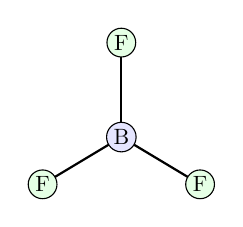
\begin{tikzpicture}[scale=1, atom/.style={circle,draw,minimum size=10pt,inner sep=1pt}]
                % Fluorine atom positions (vertices of equilateral triangle)
                \coordinate (Ftop) at (0,1.2);
                \coordinate (Fleft) at (-1, -0.6);
                \coordinate (Fright) at (1, -0.6);
                % Boron atom at the centroid
                \coordinate (B) at (0,0);
                % Bonds
                \draw[thick] (B) -- (Ftop);
                \draw[thick] (B) -- (Fleft);
                \draw[thick] (B) -- (Fright);
                % Atoms
                \node[atom, fill=blue!10] at (B) {\scalebox{0.8}{B}};
                \node[atom, fill=green!10] at (Ftop) {\scalebox{0.8}{F}};
                \node[atom, fill=green!10] at (Fleft) {\scalebox{0.8}{F}};
                \node[atom, fill=green!10] at (Fright) {\scalebox{0.8}{F}};
            \end{tikzpicture}
            \end{center}
        We want to describe the symmetries of this molecule.
            \begin{center}
            \begin{tikzpicture}[scale=1]
            % Define triangle vertices
            \coordinate (A1) at (0,1);         % top (red)
            \coordinate (B1) at (-0.866,-0.5); % bottom left (orange)
            \coordinate (C1) at (0.866,-0.5);  % bottom right (blue)
            
            % Triangle 1
            \draw[thick] (A1) -- (B1) -- (C1) -- cycle;
            \fill[red] (A1) circle(2pt);
            \fill[orange] (B1) circle(2pt);
            \fill[blue] (C1) circle(2pt);
            
            % Arrow to triangle 2
            \draw[->, thick] (1.5,0.2) -- (2.5,0.2) 
                node[midway, above, yshift=2pt] {\scalebox{0.7}{Rotate clockwise $120^\circ$}};
            \node at (2,-0.1) {\small := $r$};
    
            
            % Triangle 2 (translated copy with rotated coloring)
            \coordinate (shift1) at (4,0);
            \coordinate (A2) at ($(A1)+(shift1)$);
            \coordinate (B2) at ($(B1)+(shift1)$);
            \coordinate (C2) at ($(C1)+(shift1)$);
            
            \draw[thick] (A2) -- (B2) -- (C2) -- cycle;
            \fill[orange] (A2) circle(2pt);
            \fill[blue] (B2) circle(2pt);
            \fill[red] (C2) circle(2pt);
            
            % Arrow to triangle 3
            \draw[->, thick] (5.5,0.2) -- (6.5,0.2) 
                node[midway, above, yshift=2pt] {\scalebox{0.7}{Flip over axis of symmetry}};
            \node at (6,-0.1) {\small := $\sigma$};
        
            % Triangle 3 (another transformation)
            \coordinate (shift2) at (8,0);
            \coordinate (A3) at ($(A1)+(shift2)$);
            \coordinate (B3) at ($(B1)+(shift2)$);
            \coordinate (C3) at ($(C1)+(shift2)$);
            
            \draw[thick] (A3) -- (B3) -- (C3) -- cycle;
            \fill[orange] (A3) circle(2pt);  % Change these colors as desired
            \fill[red]    (B3) circle(2pt);
            \fill[blue]   (C3) circle(2pt);
            \end{tikzpicture}
            \end{center}
        We denote the composition of $r$ and $\sigma$ as $\sigma r$. Note that, no matter the position of our triangle, $\sigma^2$ results in no change. Consider the following moves of the same triangle:
        \begin{center}
            \begin{tikzpicture}[scale=1]
            % Define triangle vertices
            \coordinate (A1) at (0,1);         % top (red)
            \coordinate (B1) at (-0.866,-0.5); % bottom left (orange)
            \coordinate (C1) at (0.866,-0.5);  % bottom right (blue)
            
            % Triangle 1
            \draw[thick] (A1) -- (B1) -- (C1) -- cycle;
            \fill[red] (A1) circle(2pt);
            \fill[orange] (B1) circle(2pt);
            \fill[blue] (C1) circle(2pt);
            
            % Arrow to triangle 2
            \draw[->, thick] (1.5,0.2) -- (2.5,0.2) 
                node[midway, above, yshift=2pt] {\scalebox{0.7}{Rotate clockwise $240^\circ$}};
            \node at (2,-0.1) {\small := $r^2$};
    
            
            % Triangle 2 (translated copy with rotated coloring)
            \coordinate (shift1) at (4,0);
            \coordinate (A2) at ($(A1)+(shift1)$);
            \coordinate (B2) at ($(B1)+(shift1)$);
            \coordinate (C2) at ($(C1)+(shift1)$);
            
            \draw[thick] (A2) -- (B2) -- (C2) -- cycle;
            \fill[blue] (A2) circle(2pt);
            \fill[red] (B2) circle(2pt);
            \fill[orange] (C2) circle(2pt);
            
            % Arrow to triangle 3
            \draw[->, thick] (5.5,0.2) -- (6.5,0.2) 
                node[midway, above, yshift=2pt] {\scalebox{0.7}{Flip over axis of symmetry}};
            \node at (6,-0.1) {\small := $\sigma$};
        
            % Triangle 3 (another transformation)
            \coordinate (shift2) at (8,0);
            \coordinate (A3) at ($(A1)+(shift2)$);
            \coordinate (B3) at ($(B1)+(shift2)$);
            \coordinate (C3) at ($(C1)+(shift2)$);
            
            \draw[thick] (A3) -- (B3) -- (C3) -- cycle;
            \fill[blue] (A3) circle(2pt);  % Change these colors as desired
            \fill[orange]    (B3) circle(2pt);
            \fill[red]   (C3) circle(2pt);
            \end{tikzpicture}
            \end{center}

            \begin{center}
            \begin{tikzpicture}[scale=1]
            % Define triangle vertices
            \coordinate (A1) at (0,1);         % top (red)
            \coordinate (B1) at (-0.866,-0.5); % bottom left (orange)
            \coordinate (C1) at (0.866,-0.5);  % bottom right (blue)
            
            % Triangle 1
            \draw[thick] (A1) -- (B1) -- (C1) -- cycle;
            \fill[red] (A1) circle(2pt);
            \fill[orange] (B1) circle(2pt);
            \fill[blue] (C1) circle(2pt);
            
            % Arrow to triangle 2
            \draw[->, thick] (1.5,0.2) -- (2.5,0.2) 
                node[midway, above, yshift=2pt] {\scalebox{0.7}{Flip over axis of symmetry}};
            \node at (2,-0.1) {\small := $\sigma$};
    
            
            % Triangle 2 (translated copy with rotated coloring)
            \coordinate (shift1) at (4,0);
            \coordinate (A2) at ($(A1)+(shift1)$);
            \coordinate (B2) at ($(B1)+(shift1)$);
            \coordinate (C2) at ($(C1)+(shift1)$);
            
            \draw[thick] (A2) -- (B2) -- (C2) -- cycle;
            \fill[red] (A2) circle(2pt);
            \fill[blue] (B2) circle(2pt);
            \fill[orange] (C2) circle(2pt);
            
            % Arrow to triangle 3
            \draw[->, thick] (5.5,0.2) -- (6.5,0.2) 
                node[midway, above, yshift=2pt] {\scalebox{0.7}{Rotate clockwise $120^\circ$}};
            \node at (6,-0.1) {\small := $r$};
        
            % Triangle 3 (another transformation)
            \coordinate (shift2) at (8,0);
            \coordinate (A3) at ($(A1)+(shift2)$);
            \coordinate (B3) at ($(B1)+(shift2)$);
            \coordinate (C3) at ($(C1)+(shift2)$);
            
            \draw[thick] (A3) -- (B3) -- (C3) -- cycle;
            \fill[blue] (A3) circle(2pt);  % Change these colors as desired
            \fill[orange]    (B3) circle(2pt);
            \fill[red]   (C3) circle(2pt);
            \end{tikzpicture}
            \end{center}
        From this we can see $\sigma r^2 = r \sigma$. We denote the set of symmetries of this triangle as $D_3 = \{e,r,r^2 \sigma, \sigma r, \sigma r^2\}$. Given the following triangle:
            \begin{center}
                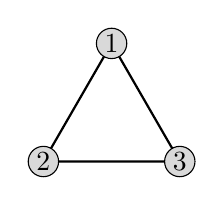
\begin{tikzpicture}[scale=1, every node/.style={circle, draw, inner sep=1pt, fill=gray!30, text=black}]

                    % Define triangle vertices
                    \coordinate (A) at (0,1);         % top
                    \coordinate (B) at (-0.866,-0.5); % bottom left
                    \coordinate (C) at (0.866,-0.5);  % bottom right
                    
                    % Draw triangle
                    \draw[thick] (A) -- (B) -- (C) -- cycle;
                    
                    % Label vertices with numbers
                    \node at (A) {1};
                    \node at (B) {2};
                    \node at (C) {3};
                    
                    \end{tikzpicture}
            \end{center}
        we can use the following notation to compute its end position:
            \begin{equation*}
            \begin{split}
                r = \bmat 1 & 2 & 3 \\ 2 & 3 & 1 \emat, \h9 \sigma = \bmat 1 & 2 & 3 \\ 1 & 3 & 2 \emat
            \end{split}
            \end{equation*}
        Note that the top row of each matrix represents the triangles initial state, and the bottom row represents where each vertex gets sent to. Observe that:
            \begin{equation*}
            \begin{split}
                r \sigma = \bmat 1 & 2 & 3 \\ 2 & 3 & 1 \emat \bmat 1 & 2 & 3 \\ 1 & 3 & 2 \emat = \bmat 1 & 2 & 3 \\ 2 & 1 & 3 \emat
            \end{split}
            \end{equation*}
        Since we work from right to left, we can see that the "1" in the matrix representing $\sigma$ gets sent to "1" by itself, and then sent to "2" by the matrix representing $r$. Similarly, the "2" in the matrix representing $\sigma$ gets sent to "3", and then sent to "1".

        We can represent these operations in a terser way. Define:
            \begin{equation*}
            \begin{split}
                r &= \bmat 1 & 2 & 3 \\ 2 & 3 & 1 \emat := (1 2 3), \\
                \sigma &= \bmat 1 & 2 & 3 \\ 1 & 3 & 2 \emat := (1)(23) = (23).
            \end{split}
            \end{equation*}
        The notation comes from the fact that $1 \rightarrow 2 \rightarrow 3 \rightarrow 1$, hence 1, 2, and $3$ are grouped together by parenthesis. We drop the 1 from the $\sigma$ notation since it is only telling us that 1 gets sent to itself. Consider:
            \begin{equation*}
            \begin{split}
                r \sigma = (123)(23).
            \end{split}
            \end{equation*}
        Working from right the left, since $2 \xrightarrow{\sigma} 3 \xrightarrow{r} 1 \xrightarrow{r} 2 \xrightarrow{r} 3$, the first part of the computation is $(23)$. We also have that $3 \xrightarrow{\sigma} 2 \xrightarrow{r} 3$. Since 3 gets sent to itself, we have that $r \sigma = (23)$. Consider:
            \begin{equation*}
            \begin{split}
                \sigma r = (23)(123)
            \end{split}
            \end{equation*}
        Since $1 \xrightarrow{\sigma} 2 \xrightarrow{\sigma} 3 \xrightarrow{r} 2 \xrightarrow{r} 3$,\h7 $2 \xrightarrow{\sigma} 3 \xrightarrow{r} 2$, \h7 and $3 \xrightarrow{\sigma} 1 \xrightarrow{\sigma} 2 \xrightarrow{r} 3$, we have that $\sigma r = (13)$. Note that we keep cycling through until we reach the closing parenthesis of $\sigma$.

        The set $D_3$ is a group under function composition. This is referred to as the \textit{dihedral group} in three elements.
    \end{example}

    \begin{example}\label{example:mod-group}
        Let $n \in \bfZ$. Define $a \sim b$ by $a \equiv b \pmod{n}$ (or, equivalently $n \mid (a-b)$). We can show that this relation is reflexive, symmetric, and transitive, hence it is an equivalence relation on $\bfZ$. For $a \in \bfZ$, define the \textit{equivalence class} of $a$ as:
            \begin{equation*}
            \begin{split}
                [a]_n 
                & := \{b \in \bfZ \mid b \equiv a \pmod{n}\} \\
                & = \{b \in \bfZ \mid n \mid (b-a) \} \\
                & = \{a + nk \mid k \in \bfZ\}.
            \end{split}
            \end{equation*}
        For each $a \in \bfZ$, the division algorithm says we can \textit{uniquely} write $a = nq + r$, for some $q,r \in \bfZ$ with $0 \leq r \leq n$. Hence all equivalence classes are given by $[0]_n$, $[1]_n$, ... $[n-1]_n$. Define:
            \begin{equation*}
            \begin{split}
                \bfZ/n\bfZ := \{[0]_n, [1]_n, ... [n-1]_n\}
            \end{split}
            \end{equation*}
        Now consider the binary operation $+:\bfZ/n\bfZ \times \bfZ/n\bfZ \rightarrow \bfZ/n\bfZ$ given by $[a]_n + [b]_n = [a+b]_n$. Note that the addition within the equivalence classes is the standard notion of integer addition, whereas the binary operation between each equivalence class is something different. Since the domain of our map "$+$" contains elements which are equivalence classes, we must verify that our map is well-defined. Let $[a_1]_n = [a_2]_n$ and $[b_1]_n = [b_2]_n$. Then $a_1 = a_2 + ns$ for some $s \in \bfZ$ and $b_1 = b_2 + nt$ for some $t \in \bfZ$. Observe that:
            \begin{equation*}
            \begin{split}
                [a_1]_n + [b_1]_n 
                & = [a_1 + b_1]_n \\
                & = [(a_2 + ns) + (b_2 + nt)]_n \\
                & = [a_2]_n + [b_2]_n + [n(s+t)]_n \\
                & = [a_2]_n + [b_2]_n.
            \end{split}
            \end{equation*}
        Thus our binary operation is well-defined. It can be shown that the set $\bfZ/n\bfZ$ is an abelian group, called the \textit{group of integers modulo $n$}.
    \end{example}

    We will now present some basic results about integers and modular arithmetic. The proofs are left out but can be found in any introductory number theory text, or online.

    \begin{theorem}
        If $a_1,a_2,...,a_n$ are integers, not all 0, then $\gcd(a_1,a_2,...,a_n)$ exists. Furthermore, there are integers $k_1,k_2,...,k_n$ such that
            \begin{equation*}
            \begin{split}
                \gcd(a_1,a_2,...,a_n) = k_1 a_1 + k_2 a_2 + ... + k_n a_n.
            \end{split}
            \end{equation*}
    \end{theorem}

    \begin{theorem}
        If $a$ and $b$ are relatively prime integers (that is, $\gcd(a,b) = 1$) and $a \mid bc$, then $a \mid c$. If $p$ is prime and $p \mid a_1 a_2 ... a_n$, then $p \mid a_i$ for some $i$.
    \end{theorem}

    Using these facts, we can generalize Example~\ref{example:mod-group} to the following theorem.

    \begin{theorem}
        Let $m>0$ be an integer and $a,b,c,d \in \bfZ$.
        \begin{enumerate}[label = (\roman*),itemsep=1pt,topsep=3pt]
            \item Congruence modulo $m$ is an equivalence relation on the set of integers $\bfZ$, which has precisely $m$ equivalence classes.
            \item If $a \equiv b \pmod{m}$ and $c \equiv d \pmod{m}$, then $a+c \equiv b + d \pmod{m}$ and $ac \equiv bd \pmod{m}$.
            \item If $ab \equiv ac \pmod{m}$ and $a$ and $m$ are relatively prime, then $b \equiv c \pmod{m}$.
        \end{enumerate}
    \end{theorem}

    The structure of these objects we've defined are extremely rich. In fact, many of the properties which we find interesting are completely independent of the elements comprising each set. This can be seen through the following definition and theorem. The proof of the theorem is left out, as it immediately follows from what has been presented earlier in this discussion.

    \begin{definition}
        A \textit{semigroup} is a nonempty set $G$ together with a binary operation on $G$ which is:
            \begin{enumerate}[label = (\arabic*),itemsep=1pt,topsep=3pt]
                \item associative: $a(bc) = (ab)c$ for all $a,b,c \in G$;
            \end{enumerate}
        A \textit{monoid} is a semigroup $G$ which contains a 
            \begin{enumerate}[label = (\arabic*),itemsep=1pt,topsep=3pt]
                \addtocounter{enumi}{1}
                \item (two-sided) identity element $e \in G$ such that $ae = ea = a$ for all $ a\in G$.
            \end{enumerate}
        A \textit{group} is a monoid $G$ such that 
            \begin{enumerate}[label = (\arabic*),itemsep=1pt,topsep=3pt]
                \addtocounter{enumi}{2}
                \item for every $a \in G$ there exists a (two-sided) inverse element $a^{-1} \in G$ such that $a^{-1}a = a a^{-1} = e$.
            \end{enumerate}
        A semigroup $G$ is said to be \textit{abelian} if its binary operation is
            \begin{enumerate}[label = (\arabic*),itemsep=1pt,topsep=3pt]
                \addtocounter{enumi}{3}
                \item commutative: $ab = ba$ for all $a,b \in \G$.
            \end{enumerate}
    \end{definition}

    \begin{theorem}
        Let $\sim$ be an equivalence relation on a monoid $G$ such that $a_1 \sim a_2$ and $b_1 \sim b_2$ imply $a_1b_1 \sim a_2 b_2$ for all $a_i,b_i \in G$. Then the set $G/\hspace{-1pt}\sim$ of all equivalence classes of $G$ under $\sim$ is a monoid under the binary operation defined by $\overline{a} \overline{b} = \overline{ab}$, where $\overline{x}$ denotes the equivalence class of $x \in G$. If $G$ is an (abelian) group, then so is $G/\hspace{-1pt}\sim$.
    \end{theorem}

    \begin{example}
        Let $X = \{1,2,3\}$. Define $S_3 := \{f:X \rightarrow X \mid f \h3\text{is bijective}\}$. It is easily verifiable that $|S_3| = 6$, and moreover that $S_3$ is a group under composition of functions. The elements of $S_3$ are:
            \begin{equation*}
            \begin{split}
                \id&: \bmat 1 & 2 & 3 \\ 1 & 2 & 3 \emat = (1), \\
                \sigma_1&: \bmat 1 & 2 & 3 \\ 2 & 1 & 3 \emat = (12), \\
                \sigma_2&: \bmat 1 & 2 & 3 \\ 3 & 2 & 1 \emat = (13), \\
                \sigma_3&: \bmat 1 & 2 & 3 \\ 1 & 3 & 2 \emat = (23), \\
                \sigma_4&: \bmat 1 & 2 & 3 \\ 2 & 3 & 1 \emat = (123), \\
                \sigma_5&: \bmat 1 & 2 & 3 \\ 3 & 1 & 2 \emat = (132). \\
            \end{split}
            \end{equation*}
        We say $S_3$ is the \textit{symmetric group} on 3 letters.
    \end{example}

    \begin{example}
        Consider the regular $n$-gon. Set $r_n$ as rotation by $\frac{2\pi}{n}$ radians  clockwise. Then $r_n^2 = r_n \circ r_n$ is a rotation by $2 \left( \frac{2\pi}{n} \right)$ radians clockwise. Similarly, $r_n^{n-1}$ is a rotation by $(n-1) \left( \frac{2\pi}{n} \right)$ radians clockwise, and $r_n^n$ is a rotation by $2\pi$ radians, hence no rotation. So $\id,r_n,r_n^2,...,r_n^{n-1}$ are distinct rigid motions. Define $C_n := \{\id,r_n,r_n^2,...,r_n^{n-1}\}$. This is an abelian group of order $n$. This is referred to as the \textit{cyclic group of order $n$}.

        Given $C_n$, if we also allow flips over an axis of symmetry, then we get $D_n$.
    \end{example}

    \begin{example}
        Define $(\bfZ/n\bfZ)^\ast := \{[a]_n \in \bfZ/n\bfZ \mid \gcd(a,n)=1\}$. This set is a group under the operation:
            \begin{equation*}
            \begin{split}
                \cdot:\bfZ/n\bfZ \times \bfZ/n\bfZ \rightarrow \bfZ/n\bfZ, \h9 [a]_n\cdot[b]_n = [ab]_n.
            \end{split}
            \end{equation*}
        The only non-trivial aspects to prove are closure under $\cdot$ and the existence of inverse elements. Let $[a]_n,[b]_n \in (\bfZ/n\bfZ)^\ast$. To show $[ab]_n \in (\bfZ/n\bfZ)^\ast$, we must prove that $\gcd(ab,n) = 1$. Suppose towards contradiction $\gcd(ab,n) \neq 1$. Then there is a prime $p$ such that $p \mid \gcd(ab,n)$. So $p \mid n$ and $p \mid ab$. Since $p$ is prime, $p \mid ab$ implies $p \mid a$ and $p \mid b$. Thus $p \mid \gcd(a,n)$ or $p \mid \gcd(b,n)$. This is a contradiction, since it implies $\gcd(a,n) \neq 1$ or $\gcd(b,n) \neq 1$; i.e., either $[a]_n \not\in (\bfZ/n\bfZ)^\ast$ or $[b]_n \not\in (\bfZ/n\bfZ)^\ast$. It must be the case that $\gcd(ab,n) = 1$.

        Given $[a]_n \in (\bfZ/n\bfZ)^\ast$, we will now show the existence of an inverse element. Since $\gcd(a,n) = 1$, there exists $s,t \in \bfZ$ such that $as + nt = 1$. Observe that:
            \begin{equation*}
            \begin{split}
                [1]_n 
                & = [as + nt]_n \\
                & = [a]_n[s]_n + [nt]_n \\
                & = [a]_n [s]_n.
            \end{split}
            \end{equation*}
        Thus $[s]_n$ is the inverse of $[a]_n$. However, is $[s]_n \in (\bfZ/n\bfZ)^\ast$? If $gcd(s,n) \neq 1$, then there is a prime $p$ such that $p \mid \gcd(s,n)$. So $p \mid s$ and $p \mid n$. Equivalently, $p \mid as$ and $p \mid nt$, so $p \mid (as + nt)$. But this contradicts $as + nt = 1$.
    \end{example}

    \begin{theorem}
        Let $G$ be any group.
        \begin{enumerate}[label = (\arabic*),itemsep=1pt,topsep=3pt]
            \item The identity element is unique.
            \item Inverses are unique.
            \item For all $a,b,c \in G$, if $ab = ac$, then $b=c$.
            \item For all $a,b \in G$, there exists $x \in G$ such that $ax=b$.
        \end{enumerate}
    \end{theorem}

\section{Subgroups and Cyclic Groups}
    \begin{definition}
        Let $(G,\ast)$ be a group. We say a nonempty subset $H \subseteq G$ is a \textit{subgroup} if $(H,\ast)$ is a group. We denote this as $H \leq G$.
    \end{definition}

    \begin{proposition}
        Let $(G,\ast)$ be a group and $H \subseteq G$. Then $H$ is a subgroup if and only if $H \neq \emptyset$ and $x\ast y^{-1} \in H$ for all $x,y \in H$.
    \end{proposition}
        \begin{proof}
            The forward direction is clear. Suppose for all $x,y \in H$ that $x \ast y^{-1} \in H$. Take $y = x$. Then $x \ast x^{-1} = e_G \in H$. Thus $H$ admits an identity. Now take $x = e$. Then $e \ast y^{-1} = y^{-1} \in H$. Thus $H$ admits inverse elements. Now take $y = y^{-1}$. Then $x \ast y \in H$, hence $H$ is closed under $\ast$. It is clear that associativity follows from this. Thus $H$ is a subgroup of $G$.
        \end{proof}

    \begin{proposition}
        Let $G$ be a group with $H,K \leq G$. Then $H \cap K \leq G$.
    \end{proposition}
        \begin{proof}
            Note that $H \cap K \neq \emptyset$ since $e_G \in H$ and $e_G \in K$. Let $x,y \in H \cap K$. Then $x,y \in H$ and $x,y \in K$. Since $H \leq G$, $xy^{-1} \in H$. Since $K \leq G$, $xy^{-1} \in K$. Thus $xy^{-1} \in H \cap K$; i.e., $H \cap K \leq G$. 
        \end{proof}

    In general $H \cup K$ is not a subgroup. Suppose $H = \{ \id , \sigma r \}$ and $K = \{id , \sigma r^2 \}$. Then $H \cup K = \{\id, \sigma r, \sigma r^2\}$, which is not closed under multiplication because $\sigma r \sigma r^2 = r^2 \not\in H \cup K$.

    \begin{definition}
        Let $G$ be a group and $a \in G$. The \textit{cyclic subgroup generated by $a$} is the set $\langle a \rangle := \{a^k \mid k \in \bfZ\}$.
    \end{definition}

    \begin{definition}
        Let $G$ be a group. We say $G$ is \textit{cyclic} if there exists a $a \in G$ such that $G = \langle a \rangle$.
    \end{definition}

    \begin{definition}
        Let $a \in G$ with $a^n = e$ for some $n \in \bfN$. If $a^m \neq e$ for all $0 < m < n$, we say $n$ is the \textit{order of $a$} and write $|a| = n$. If there is no such $n$, we say $a$ have infinite order and write $|a| = \infty$.
    \end{definition}

    \begin{proposition}***\label{prop:order-properties}
        Let $G$ be a group and $a \in G$ with $|a| = n$.
            \begin{enumerate}[label = (\arabic*),itemsep=1pt,topsep=3pt]
                \item $a^k = e$ if and only if $k \equiv 0 \pmod{n}$.
                \item $a^i = a^j$ if and only if $i \equiv j \pmod{n}$.
                \item $|\langle a \rangle| = |a|$.
                \item $\langle a^k \rangle = \langle a \rangle$ if and only if $\gcd(k,n) = 1$.
                \item $\langle a^k \rangle = \langle a^{\gcd(k,n)} \rangle$.
                \item ***$|a^k| = \frac{n}{\gcd(k,n)}$.
            \end{enumerate}
    \end{proposition}
        \begin{proof}
            (1) This is a special case of (2). \nl
            
            \noindent (2) ($\Rightarrow$) If $a^i = a^j$, then $a^{i-j} = e$. Apply the division algorithm to $i-j$ and $n$. Then there exists unique $q,r \in \bfZ$ such that $i-j = nq + r$, where $0 \leq r < n$. Thus:
                \begin{equation*}
                \begin{split}
                    e 
                    & = a^{i-j} \\
                    & = a^{nq + r} \\
                    & = a^{nq}a^r \\
                    & = a^r.
                \end{split}
                \end{equation*}
            But since $r < n$, and $n$ is the smallest number such that $a^n = e$, it must be the case that $r = 0$. Thus $i-j = nq$; i.e., $i \equiv j \pmod{n}$.

            ($\Leftarrow$) If $i \equiv j \pmod{n}$, then $i = j + nq$ for some $q \in \bfZ$. Thus $a^i = a^{j + nq} = a^j a^{nq} = a^j$. \nl
            
            \noindent (3) Suppose $k > n$. Apply the division algorithm to $k$ and $n$. There exists $q,r \in \bfZ$ such that $k = nq + r$, $0 \leq r < n$. Thus $a^k = a^{nq+r} = a^r$, $0 \leq r < n$. If $a^i = a^j$ where $0 \leq i < n$ and $0 \leq j < n$, then $a^{i-j} = e$. Clearly $i-j < n$, and since $n$ is the smallest number such that $a^n = e$, it must be the case that $i - j = 0$. Hence $i = j$. From these two observations, we can deduce that $\langle a \rangle = \{e,a,a^2,...,a^{n-1}\}$. Thus $|\langle a \rangle| = n = |a|$. \nl
            
            \noindent (4) This is a special case of (5) \nl
            
            \noindent (5) Let $a^b \in \langle a^k \rangle$. Then $a^b = a^{ky}$ for some $y \in \bfZ$. Note that $\div{\gcd (n,k)}{n}$ and $\div{\gcd (n,k)}{k}$. So there exists $u \in \bfZ$ such that $\gcd(n,k)\cdot u = k$. This gives:
                \begin{equation*}
                \begin{split}
                    a^b 
                    & = a^{ky} \\
                    & = a^{\gcd(n,k)\cdot u y} \\
                    & = \left(a^{\gcd(n,k)}\right)^{uy} \in \langle a^{\gcd(n,k)} \rangle.
                \end{split}
                \end{equation*}
            Hence $\langle a^k \rangle  \subseteq \langle a^{\gcd(n,k)} \rangle$. Now let $a^b \in \langle a^{\gcd(n,k)} \rangle$ Then $a^b = a^{\gcd(n,k) \cdot y}$ for some $y \in \bfZ$. There exists $s,t \in \bfZ$ such that $\gcd(n,k) = ns + kt$. This gives: 
                \begin{equation*}
                \begin{split}
                    a^b 
                    & = a^{\gcd(n,k)\cdot y} \\
                    & = a^{nsy + kty} \\
                    & = a^{nsy} a^{kty} \\
                    & = \left(a^k\right)^{ty} \in \langle a^k \rangle.
                \end{split}
                \end{equation*}
            Hence $\langle a^{\gcd(n,k)} \rangle \subseteq \langle a^k \rangle$. Thus $\langle a^k \rangle = \langle a^{\gcd(k,n)} \rangle$. \nl
            
            \noindent (6) ***First note that:
                \begin{equation*}
                \begin{split}
                    \left( a^k \right)^{\frac{n}{\gcd(k,n)}} 
                    & = \left(a^n\right)^\frac{k}{\gcd(k,n)} \\
                    & = e^\frac{k}{\gcd(k,n)} \\
                    & = e.
                \end{split}
                \end{equation*}
            Now suppose $0 < m < \frac{n}{\gcd(k,n)}$. Then $0 < m \cdot \gcd(k,n) < n$. Since $|a| = n$, it must be the case that $\left( a^{\gcd(k,n)} \right)^m \neq e$. We showed in (4) that $\langle a^k \rangle = \langle a^{\gcd(k,n)} \rangle$. Since $\left( a^{\gcd(k,n)} \right)^m \in \langle a^{\gcd(k,n)} \rangle$, it must be the case that $\left( a^k \right)^m = \left( a^{\gcd(k,n)} \right)^m \neq e$. Thus $\frac{n}{\gcd(k,n)}$ is the smallest number such that $\left( a^k \right)^{\frac{n}{\gcd(k,n)}} = e$, hence $|a^k| = \frac{n}{\gcd(k,n)}$.
        \end{proof}

    \begin{theorem}***
        Let $G$ be a finite cyclic group.
            \begin{enumerate}[label = (\arabic*),itemsep=1pt,topsep=3pt]
                \item Any subgroup of $G$ is cyclic.
                \item If $H \leq G$, then $\div{|H|}{|G|}$
                \item ***For any divisor $\div{d}{|G|}$, there is a unique subgroup $H \leq G$ so that $|H| = d$.
            \end{enumerate}
    \end{theorem}
        \begin{proof}
            (1) Let $H \leq G$ be nontrivial. Since $G$ is cyclic, there exists $a \in G$ such that $\langle a \rangle = G$. Let $m$ be the smallest positive integer so that $a^m \in H$. It is clear that $\langle a^m \rangle \subseteq H$. Let $a^n \in H$ with $n > 0$. Write $n = mq + r$ for some $q,r \in \bfZ$, $0 \leq r  < m$. Then:
                \begin{equation*}
                \begin{split}
                    a^r 
                    & = a^{n-mq} \\
                    & = a^n (a^m)^{-q} \\
                    & \in H.
                \end{split}
                \end{equation*}
            Since $m$ is the smallest positive integer such that $a^m \in H$, it must be the case that $r = 0$. Thus $a^n = (a^m)^q \in \langle a^m \rangle$; i.e., $H \subseteq \langle a^m \rangle$. Since $H = \langle a^m \rangle$, $H$ is cyclic. \nl
            
            \noindent (2) Since $G$ is cyclic, there exists $a \in G$ such that $\langle a \rangle = G$. Let $m$ be the smallest positive integer such that $a^m \in H$. By the same construction in (1) we have $H = \langle a^m \rangle$. By Proposition~\ref{prop:order-properties}, we have:
                \begin{equation*}
                \begin{split}
                    |H|
                    & = |\langle a^m \rangle| \\
                    & = |a^m| \\
                    & = \frac{|a|}{\gcd(m,|a|)} \\
                    & = \frac{|\langle a \rangle|}{\gcd(m,|a|)} \\
                    & = \frac{|G|}{\gcd(m,|a|)}.
                \end{split}
                \end{equation*}
            Since $|H| \cdot \gcd(m,|a|) = |G|$, we've shown $\div{|H|}{|G|}$. \nl
            
            \noindent (3) ***
        \end{proof}

\section{Homomorphisms and Isomorphisms}
    \begin{definition}
        Let $G$ and $H$ be groups. A \textit{group homomorphism} is a map $\varphi:G \rightarrow H$ that satisfies $\varphi(g_1g_2) = \varphi(g_1)\varphi(g_2)$ for all $g_1,g_2 \in G$. If in addition $\varphi$ is bijective, we say that $\varphi$ is a \textit{group isomorphism}. If $\varphi$ is a group isomorphism between $G$ and $H$, we say $G$ is \textit{isomorphic} to $H$, and write $G \cong H$.
    \end{definition}

    \begin{example}
        Let $G$ be a cyclic group of order $n$. Then there exists $a \in G$ such that $\langle a \rangle = G$. Define $\varphi:\bfZ/n\bfZ \rightarrow G$ by $[x]_n \mapsto a^x$. This is an isomorphism.
    \end{example}

    \begin{proposition}
        Let $\varphi:G \rightarrow H$ be a homomorphism. Then for all $g \in G$:
            \begin{enumerate}[label = (\arabic*),itemsep=1pt,topsep=3pt]
                \item $\varphi(e_G) = e_H$
                \item $\varphi(g^n) = \varphi(g)^n$
                \item $\div{|\varphi(g)}{|g|}$
                \item $\varphi(g^{-1})=\varphi(g)^{-1}$
            \end{enumerate}
    \end{proposition}
        \begin{proof}
            We only prove (3). Let $|g| = m$. We have:
                \begin{equation*}
                \begin{split}
                    \varphi(g)^m 
                    & = \varphi(g^m) \\
                    & = \varphi(e_G) \\
                    & = e_H.
                \end{split}
                \end{equation*}
            Since $\varphi(g)^m = e_H$, we have $\div{|\varphi(g)}{m}$.
        \end{proof}

    \begin{definition}
        Let $\varphi:G \rightarrow H$ be a group homomorphism.
        \begin{enumerate}[label = (\arabic*),itemsep=1pt,topsep=3pt]
            \item The \textit{kernel} of $\varphi$ is $\ker \varphi = \{g \in G \mid \varphi(g) = e_H\}$.
            \item The \textit{image} of $\varphi$ is $\Image \varphi = \{\varphi(g) \mid g \in G\}$.
        \end{enumerate}
    \end{definition}

    \begin{proposition}
        Let $\varphi:G \rightarrow H$ be a group homomorphism.
            \begin{enumerate}[label = (\arabic*),itemsep=1pt,topsep=3pt]
                \item $\ker \phi \leq G$
                \item $\Image \phi \leq H$
                \item $\ker \varphi = \{e_G\}$ if and only if $\varphi$ is injective.
                \item $\Image \varphi = H$ if and only if $\varphi$ is surjective.
            \end{enumerate}
    \end{proposition}
        \begin{proof}
            (1) Note that $\ker \varphi \neq \emptyset$ since $\varphi(e_G) = e_H$. Let $g_1,g_2 \in \ker \varphi$. Observe that:
                \begin{equation*}
                \begin{split}
                    \varphi(g_1 g_2^{-1})
                    & = \varphi(g_1)\varphi(g_2^{-1}) \\
                    & = \varphi(g_1)\varphi(g_2)^{-1} \\
                    & = e_H.
                \end{split}
                \end{equation*}
            Thus $g_1g_2^{-1}\in \ker \varphi$, giving $\ker \varphi$ as a subgroup of $G$.\nl
            
            \noindent (2) Let $h_1,h_2 \in \Image \varphi$. Then there exists $g_1,g_2 \in G$ with $\varphi(g_1) = h_1$ and $\varphi(g_2) = h_2$. We have:
                \begin{equation*}
                \begin{split}
                    h_1h_2^{-1}
                    & = \varphi(g_1)\varphi(g_2)^{-1} \\
                    & = \varphi(g_1)\varphi(g_2^{-1}) \\
                    & = \varphi(g_1g_2^{-1}).
                \end{split}
                \end{equation*}
            Whence $h_1h_2^{-1} \in \Image \varphi$, giving $\Image \varphi$ as a subgroup of $H$. \nl
            
            \noindent (3) Let $\ker \varphi = \{0\}$. Let $g_1,g_2 \in G$ and suppose $\varphi(g_1) = \varphi(g_2)$. Then $\varphi(g_1)\varphi(g_2)^{-1} = \varphi(g_1g_2^{-1}) = e_H$. It must be that $g_1g_2^{-1} = e_G$, giving $g_1 = g_2$. Conversely, suppose $\varphi$ is injective and let $g \in \ker \varphi$. Then $\varphi(g) = e_H = \varphi(e_G)$. Hence $g = e_G$, establishing $\ker \varphi = \{e_G\}$. \nl
            
            \noindent (4) This is by definition of surjectivity.
        \end{proof}

    \begin{example}
        The map $\varphi:\bfZ \rightarrow \bfZ/2\bfZ$ defined by $\varphi(a) = [a]_2$ is a well-defined homomorphism. In particular:
            \begin{equation*}
            \begin{split}
                \ker \varphi 
                & = \{m \in \bfZ \mid \varphi(m) = [0]_2 \} \\
                & = \{m \in \bfZ \mid [m]_2 = [0]_2 \} \\
                & = \{m \in \bfZ \mid m \equiv 0 \pmod{2}\} \\
                & = \{m \in \bfZ \mid m = 2k,\h2 k \in \bfZ\} \\
                & = 2\bfZ.
            \end{split}
            \end{equation*}
    \end{example}

    \begin{example}
        The map $\varphi:\bfZ/10\bfZ \rightarrow \bfZ/2\bfZ$ defined by $\varphi([a]_{10}) = [a]_2$ is a well-defined homomorphism. In particular, one can prove that $\ker \varphi = \{[m]_{10} \in \bfZ/10\bfZ \mid [m]_2 = [0]_2 \} = 2\bfZ/10\bfZ$.
    \end{example}

\section{Cosets, Normal Subgroups, and Quotient Groups}
    \begin{definition}
        Let $G$ be a group, $g \in G$ and $H \leq G$. A left (resp. right) \textit{coset} of $g$ is the set $gH = \{gh \mid h \in H\}$ (resp. $Hg = \{hg \mid h \in H\}$). The collection of left (resp. right) cosets is denoted $G/H = \{gH \mid g \in G\}$ (resp. $H\setminus G = \{Hg \mid g \in G\}$).
    \end{definition}



    